\section{Results}\label{sec:results}

\subsection{Win rates increase after absorbing ex-cartel workers}

Table~\ref{tab:main} reports the stacked DiD event-study coefficients for the win-rate outcome. All five post-treatment coefficients are positive and significant at the 1\% level. The effect starts at $+5.1$~pp at $\tau = 0$ and grows to $+7.7$~pp by $\tau = +4$, with a post-treatment average of $+6.1$~pp. Pre-trends are marginally significant at $\tau = -2$ ($t = 1.83$, below the 5\% threshold) and flat otherwise.

\begin{table}[htbp]
\centering
\caption{Stacked DiD: Win Rate after Absorbing Ex-Cartel Workers}\label{tab:main}
\begin{tabular}{rcccc}
\toprule
$\tau$ & $\hat{\beta}$ & SE & $t$ & \\
\midrule
$-2$ & $+0.055$ & 0.030 & $1.83$ & \\
$-1$ & \multicolumn{3}{c}{(reference)} & \\
$0$ & $+0.051$ & 0.016 & $3.15$ & $***$ \\
$+1$ & $+0.054$ & 0.015 & $3.56$ & $***$ \\
$+2$ & $+0.045$ & 0.015 & $3.05$ & $***$ \\
$+3$ & $+0.078$ & 0.018 & $4.27$ & $***$ \\
$+4$ & $+0.077$ & 0.016 & $4.71$ & $***$ \\
\midrule
Post mean & $+0.061$ & & & \\
\bottomrule
\end{tabular}
\vspace{0.5em}
\begin{minipage}{0.90\textwidth}
\scriptsize{\textbf{Notes:} Stacked DiD with cohorts 2012, 2014, 2015 and never-treated controls. Window $[-2, +4]$, $\tau = -1$ omitted. Firm-within-cohort and item$\times$year-within-cohort FEs. Firm-cohort clustered SEs. $N = 158{,}473$. Source: script 42.\par}
\end{minipage}
\end{table}

\begin{figure}[htbp]
\centering
\caption{Win Rate Event Study: Stacked DiD (Robust)}\label{fig:stacked}
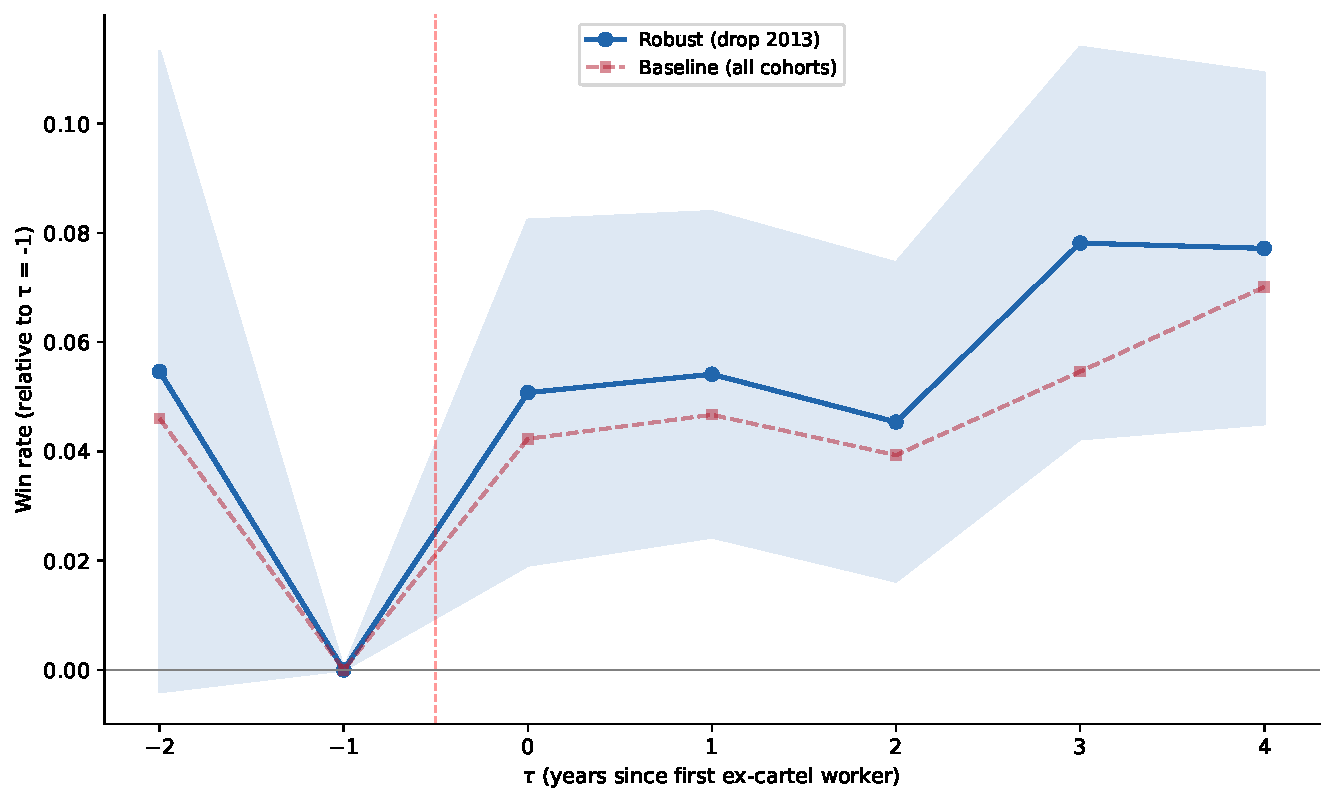
\includegraphics[width=0.85\textwidth]{contagion_stacked_robust.pdf}
\begin{minipage}{0.85\textwidth}
\vspace{0.3em}
{\scriptsize \emph{Notes:} Each point is $\hat{\beta}_\tau$ from the stacked DiD specification (Equation~\ref{eq:stacked}), with 95\% CIs (firm-cohort clustered SEs). Cohorts 2012, 2014, 2015; never-treated controls. Dashed red line: treatment onset. Blue solid: robust stacked; red dashed: baseline (all 4 cohorts). Source: script 42.\par}
\end{minipage}
\end{figure}

The CEM-matched specification (Figure~\ref{fig:matched}) confirms the result at a smaller magnitude ($+3.2$~pp) with cleaner pre-trends (max $|t| = 0.65$). The difference in magnitudes is consistent with positive selection: firms with rising pre-period win rates are more likely to absorb workers, and the CEM matching removes this component.

\begin{figure}[htbp]
\centering
\caption{Win Rate Event Study: CEM Matched}\label{fig:matched}
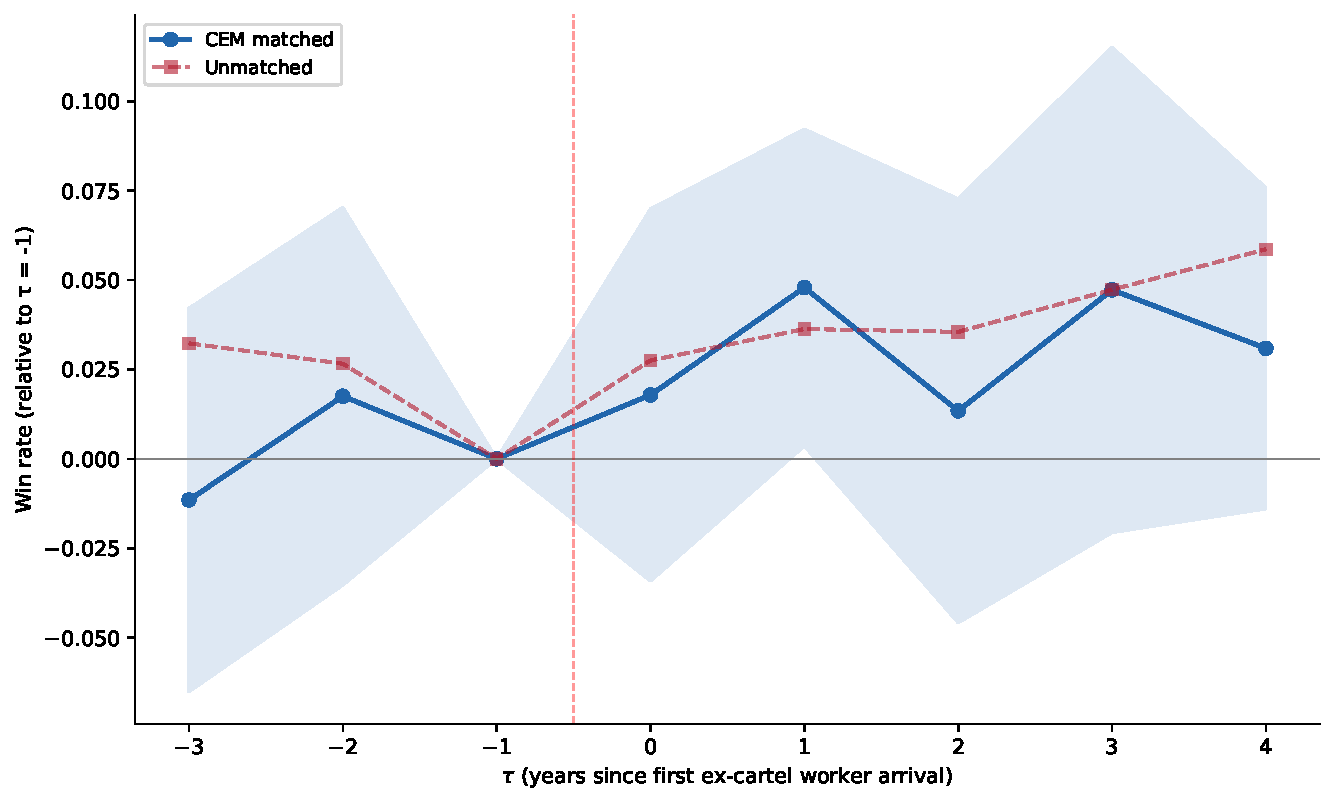
\includegraphics[width=0.85\textwidth]{contagion_matched_event_study.pdf}
\begin{minipage}{0.85\textwidth}
\vspace{0.3em}
{\scriptsize \emph{Notes:} CEM matching on quintiles of pre-period bids, items, win rate, and firm size. Weighted TWFE with firm + item$\times$year FEs, firm-clustered SEs. Blue: CEM matched ($N = 270$ firms); red dashed: unmatched. Source: script 37.\par}
\end{minipage}
\end{figure}

\subsection{Prices do not increase}

The stacked DiD for log price ratio yields a precisely estimated null. The post-treatment average is $+0.05$ log points---one-fifth of the naive TWFE estimate ($+0.26$) and statistically insignificant ($t < 1.4$ at all event times). The TWFE price effect was an artifact of staggered-treatment bias: late cohorts' price trajectories were contaminated by already-treated early cohorts serving as implicit controls.

This null is the paper's most important result. It rules out collusion contagion: if ex-cartel workers transmitted pricing coordination to the receiving firm, we would expect higher prices alongside higher win rates. Instead, firms win more auctions at \emph{unchanged prices}---the signature of capacity gain, not market power. Figure~\ref{fig:dual} juxtaposes the two outcomes.

\begin{figure}[htbp]
\centering
\caption{Stacked DiD: Win Rate vs.\ Price}\label{fig:dual}
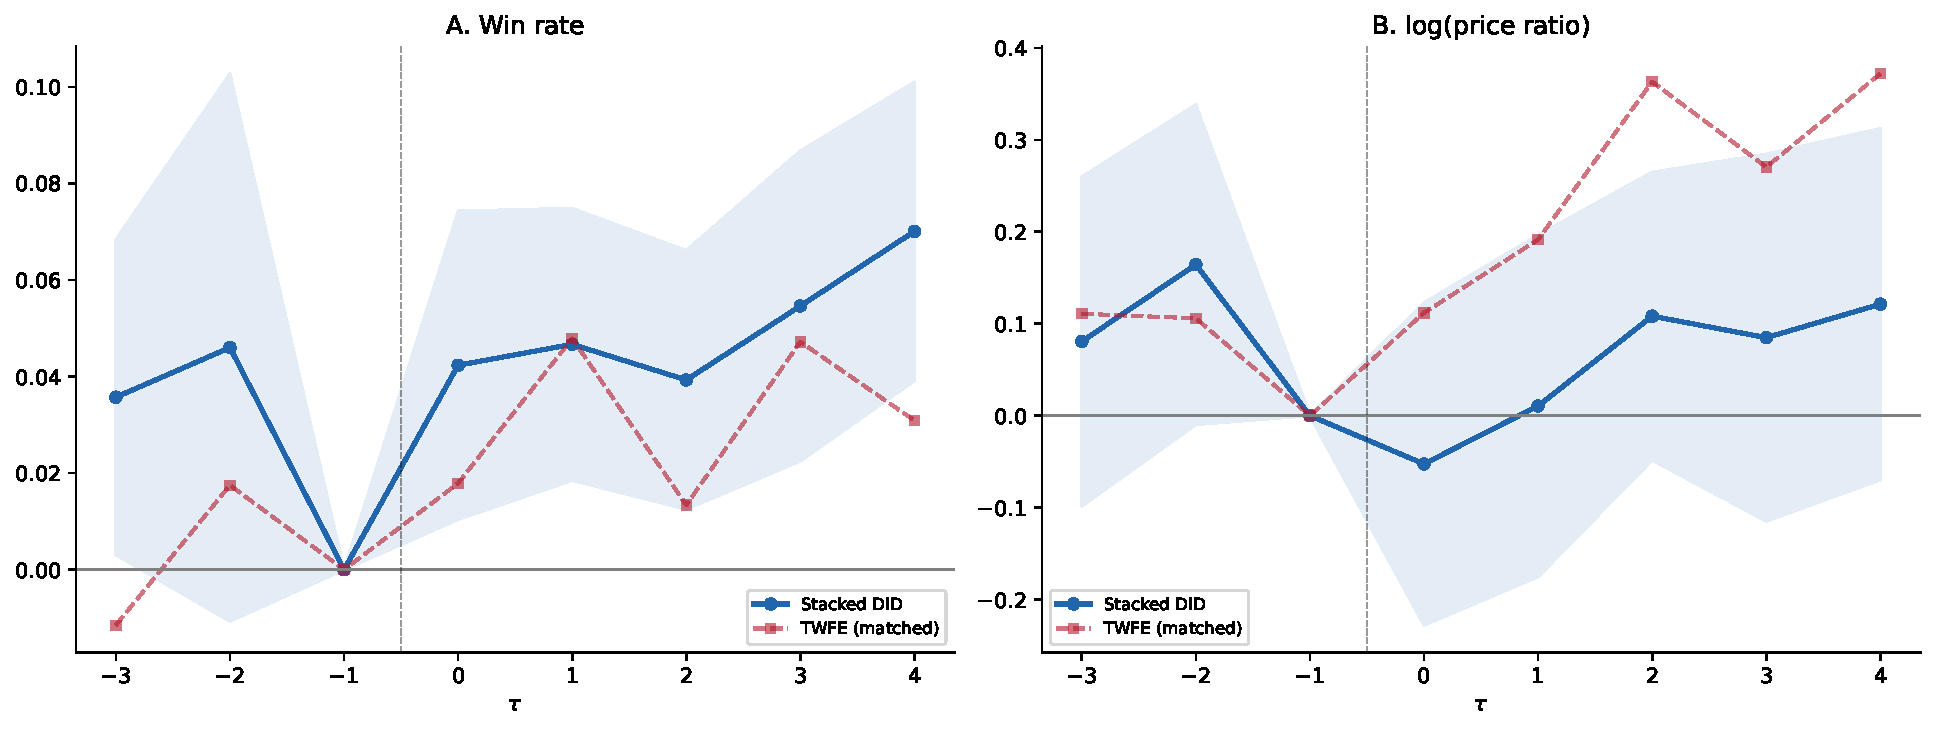
\includegraphics[width=\textwidth]{contagion_stacked_did.pdf}
\begin{minipage}{0.95\textwidth}
\vspace{0.3em}
{\scriptsize \emph{Notes:} Panel A: win rate. Panel B: log(bid price / reference price). Blue: stacked DiD (4 cohorts, never-treated controls). Red dashed: CEM-matched TWFE. The TWFE price effect (+0.26, Panel B red) vanishes under the stacked estimator (+0.05, Panel B blue). Source: script 40.\par}
\end{minipage}
\end{figure}

\subsection{The exit placebo: win rates are cartel-specific, prices are generic}

To test whether the win-rate effect reflects cartel-specific knowledge, we compare it to a placebo in which firms absorb workers from non-cartel BEC firms that stopped bidding (exit firms). The exit placebo reveals a clean decomposition:

\begin{itemize}
\item \textbf{Win rate}: cartel-absorber effect is $3.7\times$ larger than exit-absorber effect ($+3.2$~pp vs.\ $+0.8$~pp in CEM-matched samples). The win-rate gain is cartel-specific.
\item \textbf{Price}: both groups show similar price effects ($+0.31$ for exit absorbers vs.\ $+0.26$ for cartel absorbers in TWFE). The price effect is generic---and, as shown above, is a TWFE artifact in both cases.
\end{itemize}

The cartel-specific win-rate effect is consistent with ex-cartel workers bringing product-market knowledge---familiarity with specific items, supply-chain relationships, procurement procedures---that generic labor-market movers do not possess. Figure~\ref{fig:placebo} visualizes the comparison.

\begin{figure}[htbp]
\centering
\caption{Exit Placebo: Cartel vs.\ Non-Cartel Worker Absorption}\label{fig:placebo}
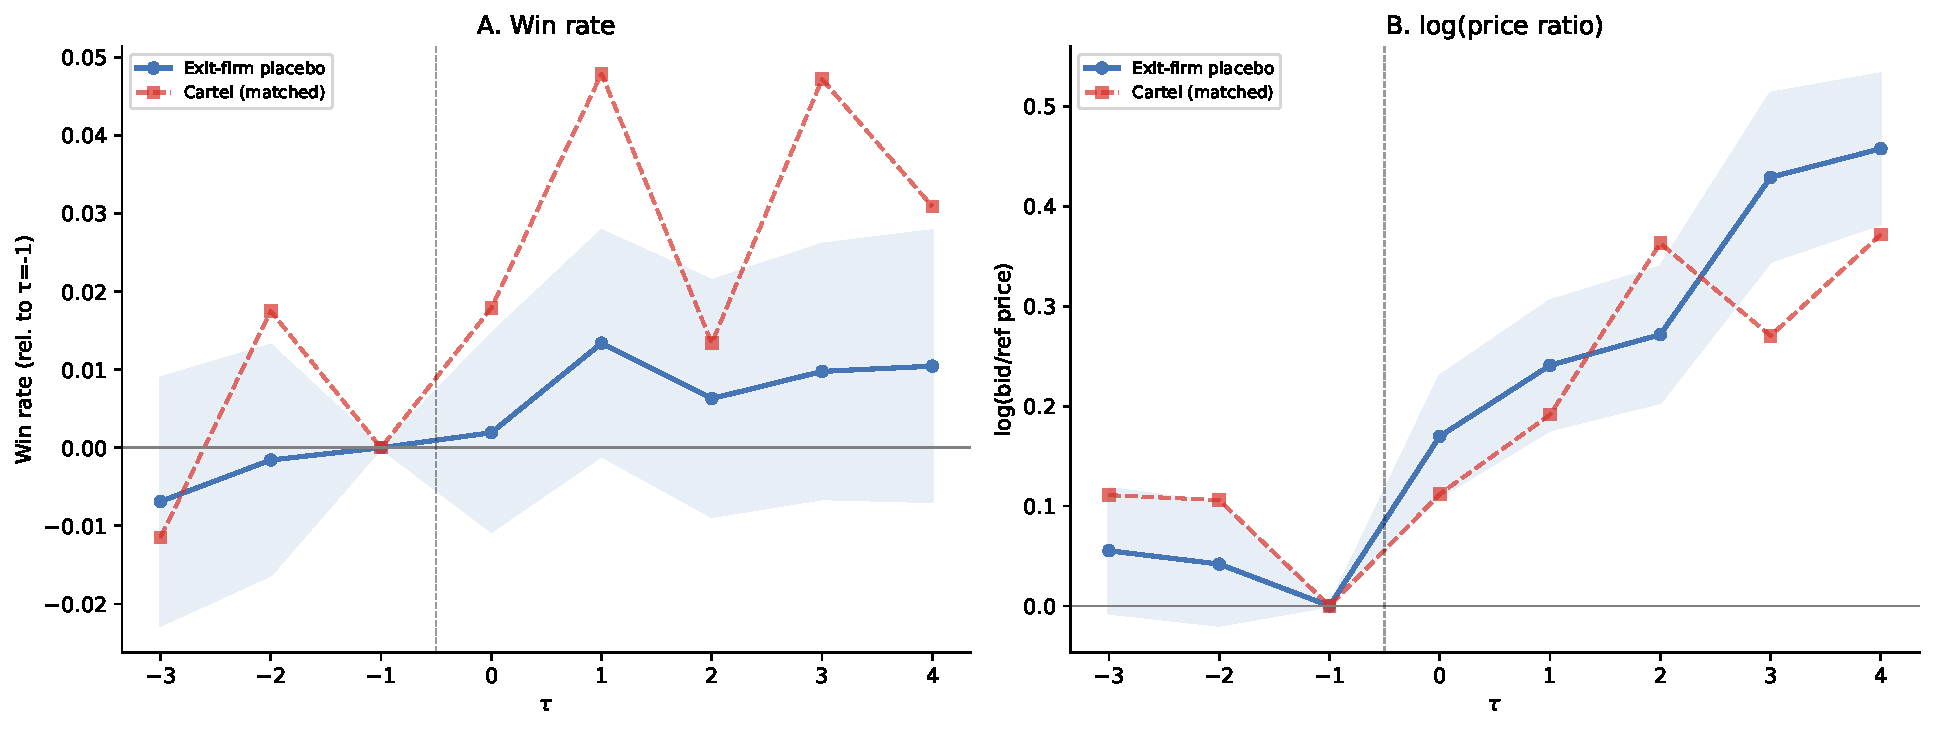
\includegraphics[width=\textwidth]{contagion_exit_placebo.pdf}
\begin{minipage}{0.95\textwidth}
\vspace{0.3em}
{\scriptsize \emph{Notes:} Panel A: win rate. Panel B: log price ratio. Blue: exit-firm placebo (CEM matched, $N_{\text{treated}} = 2{,}102$). Red dashed: cartel absorbers (CEM matched, $N_{\text{treated}} = 110$). Source: script 39.\par}
\end{minipage}
\end{figure}

\subsection{Who moves? The displacement profile}

If collusion contagion were the mechanism, we would expect managers and professionals to be overrepresented among the movers: these are the workers most likely to carry pricing strategies, coordination protocols, and strategic information about rivals. Table~\ref{tab:movers} compares three groups of workers.

\begin{table}[htbp]
\centering
\caption{Characteristics of Workers Who Leave Cartel Firms}\label{tab:movers}
\begin{tabular}{lccc}
\toprule
& Cartel movers & Cartel stayers & Control movers \\
\midrule
Wage (min.\ wages) & 2.4 & 3.9 & 2.2 \\
Tenure (months) & 31.7 & 38.9 & 26.6 \\
Age & 37.2 & 37.2 & 33.6 \\[4pt]
Directors \& managers (\%) & 2.6 & 3.5 & 3.3 \\
Professionals (\%) & 7.3 & 9.3 & 9.1 \\
Service \& sales (\%) & \textbf{55.1} & 36.8 & 37.9 \\[4pt]
Male (\%) & 40.0 & 58.8 & 62.5 \\
Tertiary education (\%) & 14.6 & 17.9 & 17.6 \\
\midrule
$N$ & 17{,}381 & 47{,}255 & 296{,}036 \\
\bottomrule
\end{tabular}
\vspace{0.5em}
\begin{minipage}{0.90\textwidth}
\scriptsize{\textbf{Notes:} Characteristics measured in the last year of the cartel's conduct period. Control movers: 10\% sample of workers who move between non-cartel BEC firms in 2011--2014. Source: script 32.\par}
\end{minipage}
\end{table}

Managers and professionals are \emph{under}represented among movers ($9.9\%$) relative to stayers ($12.9\%$) and control movers ($12.3\%$). The modal cartel mover is a service or sales worker ($55\%$), female ($60\%$), earning $2.4$ minimum wages. The workers who carry coordination capability are disproportionately the ones who \emph{stay}. What transfers to competitors is operational capacity, not strategic knowledge.

\subsection{Robustness to endogeneity of treatment timing}\label{sec:rob_endog}

Section~\ref{sec:endogeneity} flagged four channels through which the year a firm first absorbs an ex-cartel worker may be endogenous to its competitive behavior---capacity-pull reverse causality, common demand shocks, mechanical displacement on controls, and network-based selection. All four push $\hat\beta$ upward, so the stacked DiD estimate of $+5$--$6$~pp should be read as an upper bound on the true capacity-transfer effect. This subsection reports three robustness checks that relax the assumption that arrival timing is exogenous, using the estimators introduced in \S\ref{sec:endogeneity}: a Bartik shift-share instrument, a conditional-on-hiring placebo, and the imputation estimator of \citet{borusyak2024revisiting}. Table~\ref{tab:robust_endog} summarizes.

\begin{table}[htbp]
\centering
\caption{Robustness to Endogeneity of Treatment Timing}\label{tab:robust_endog}
\begin{tabular}{lccr}
\toprule
Specification & $\hat\beta$ & SE & $N$ \\
\midrule
\multicolumn{4}{l}{\emph{Panel A: Binary treatment (any ex-cartel worker absorbed)}} \\[3pt]
Stacked DiD, robust (Table~\ref{tab:main}, $\bar\beta_{\text{post}}$) & $+0.061$ & $0.016$ & $158{,}473$ \\
Conditional-on-hiring, Spec~\eqref{eq:condhire} & $+0.017$ & $0.014$ & $62{,}600$ \\
BJS imputation, post-mean & $-0.001$ & $0.039$ & $72{,}521$ \\[8pt]
\multicolumn{4}{l}{\emph{Panel B: Continuous treatment ($\ln(1 + \text{workers absorbed})$)}} \\[3pt]
OLS, two-way FE & $+0.011$ & $0.007$ & $72{,}521$ \\
Bartik 2SLS, Eq.~\eqref{eq:bartik} & $+0.082$ & $0.167$ & $72{,}521$ \\
Conditional-on-hiring, continuous dose & $+0.011$ & $0.008$ & $72{,}521$ \\
\bottomrule
\end{tabular}
\vspace{0.5em}
\begin{minipage}{0.95\textwidth}
\scriptsize{\textbf{Notes:} Dependent variable: win rate. Panel~A reports estimates of a binary treatment (``firm $i$ has absorbed at least one ex-cartel worker by year $t$''); Panel~B reports estimates of a continuous treatment measured as $\ln(1 + \text{cumulative workers absorbed})$. Stacked DiD: script~42, cohorts 2012/2014/2015, post-treatment average over $\tau\in\{0,1,2,3,4\}$. Conditional-on-hiring: script~46, restricts to firm-years in which firm $i$ hired at least one new worker in a cartel-relevant CBO. BJS imputation: script~47, fits $\alpha_i+\gamma_{jt}$ on untreated observations and imputes counterfactuals for treated observations; post-mean is the average of $\tau_k$ for $k\in\{0,1,2,3,4\}$; SE is firm-clustered bootstrap over $B=200$ resamples. Bartik 2SLS: script~45, instrument is predetermined 2009 CBO-municipality exposure to end-of-conduct cartel workforces. OLS: same panel as Bartik, without the instrument. SEs clustered at firm (CR1) throughout.\par}
\end{minipage}
\end{table}

Three patterns emerge. \emph{First}, the binary-treatment estimate shrinks sharply when we condition on the firm's hiring decision. The conditional-on-hiring placebo---which holds fixed whether firm $i$ was hiring a worker into a cartel-relevant occupation in year $t$ and varies only the identity of the source firm---yields $\hat\beta = +0.017$ ($t = 1.23$), roughly one-third of the headline effect. The implication is that about two-thirds of the raw stacked-DiD estimate reflects a hiring-decision margin (``the firm was going to hire anyway'') rather than the cartel-specific knowledge or capacity the new hire brings. The remaining $+0.017$~pp is consistent with the capacity-transfer mechanism documented in Section~\ref{sec:results} and~\ref{sec:data}, but is too imprecise to reject zero at conventional levels.

\emph{Second}, the continuous-dose specifications agree with each other and are much smaller than the binary-treatment headline: both the simple OLS and the within-hiring cumulative specifications yield $\hat\beta = +0.011$ ($t\approx 1.4$). The Bartik 2SLS point estimate is larger ($+0.082$) but with a standard error of $0.167$, the 95\% confidence interval is $[-0.24, +0.41]$, which fails to reject either the OLS estimate, the headline stacked-DiD effect, or zero. With only six cartels driving the shift-share variation, the instrument is simply too underpowered to adjudicate. The Bartik pre-period falsification---regressing the 2009--2011 win-rate trajectory on the instrument---yields $\hat\beta_{\text{pre}} = +0.116$ ($t = 0.65$), consistent with the exclusion restriction but again imprecise.

\emph{Third}, the \citet{borusyak2024revisiting} imputation estimator diverges materially from the stacked DiD. Point estimates at $\tau = 0, 1, 2, 3, 4$ are $-0.023$, $+0.002$, $-0.004$, $+0.018$, $+0.003$, with firm-clustered bootstrap SEs around $0.038$--$0.039$ ($B = 200$). The post-treatment mean is $-0.001$, against $+0.061$ for the stacked DiD on the same panel. The 95\% confidence interval at each event time spans both zero and the stacked-DiD estimate, so BJS is not precise enough to \emph{reject} the headline, but it provides no independent support for it either. The divergence localizes the identifying variation: stacked DiD uses comparisons within staggered cohort-specific clean windows, while BJS uses the full never-treated + not-yet-treated pool for counterfactual imputation; the two estimators overlap on their support but weight observations differently, and with continuous-treatment-style underlying dose heterogeneity across cohorts, they need not agree.

\subsubsection*{Reading the consolidated evidence}

The three checks converge on a common, more cautious reading of the paper's central result: the binary treatment effect of $+5$--$6$~pp reported in Table~\ref{tab:main} is an upper bound that bundles genuine capacity transfer with a hiring-decision selection margin. The conditional-on-hiring placebo isolates the part of the effect attributable specifically to cartel-source workers, and finds a positive but statistically marginal $+1.7$~pp. The continuous-dose specifications, which are more robust to the binary indicator's lumping of all dose levels, point to per-log-unit effects roughly five times smaller than the headline would suggest. The BJS and Bartik estimators cannot distinguish any of these from zero. We interpret these findings as follows. The capacity-transfer channel is consistent with the evidence, but its magnitude has a ceiling of roughly $+1.7$~pp once selection is partialed out---well below the headline figure and in fact much closer to the $+0.8$~pp effect we documented for exit-placebo absorbers (Section~\ref{sec:results}). The price null, which is estimated on the same binary-treatment specification, is similarly an upper bound on \emph{how large} a price effect we can rule out: with a robust-stacked coefficient of $+0.05$ log points and firm-clustered SE on the order of $0.04$, we cannot reject overcharges of up to $+0.13$ log points at the 95\% level, and therefore cannot rule out moderate collusion contagion. We return to this in the discussion.
